\section{Linear complexity RPE
implementation}

In this section we will detail how the relative positional encoding
 proposed by \citet{shaw2018selfattention}
can in fact be computed with linear complexity. The $S_{rel}$ matrix of scores is computed as
${S_{rel}}_{ij} = \vec{Q_i} \cdotp \vec{RP}_{clip(i-j, -k, k)}$. In figure \ref{fig:S_rel} the colors represent the index of the query and the number the
index of the relative position.

\begin{figure}
\centering
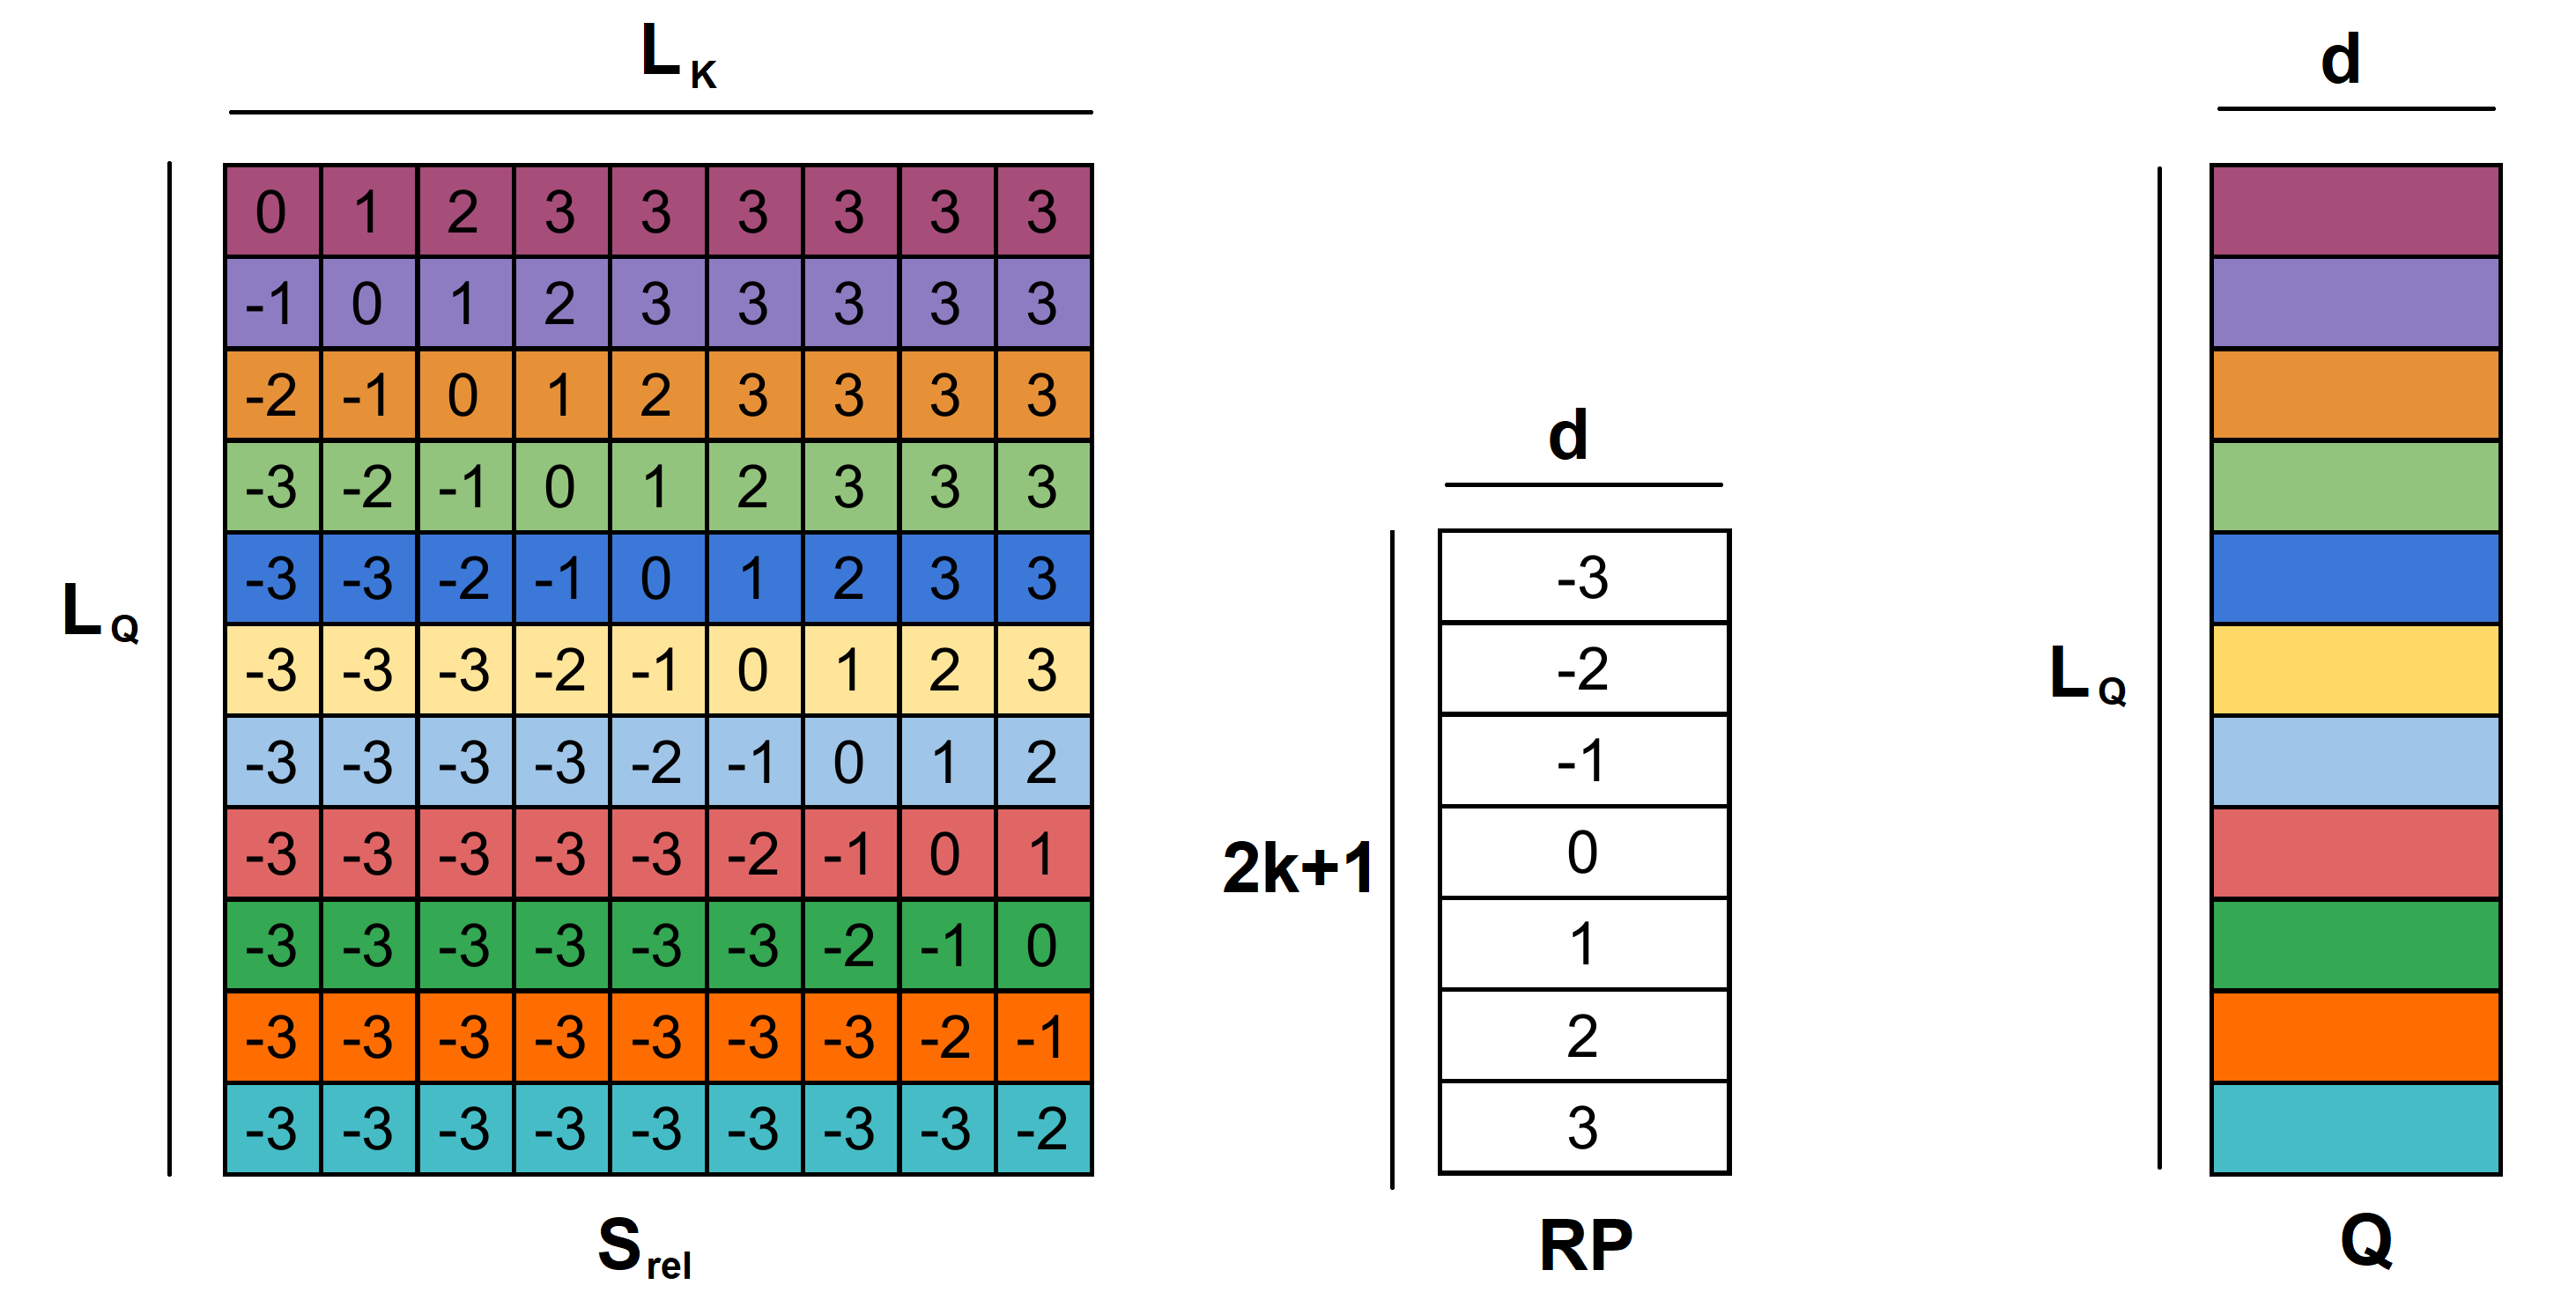
\includegraphics[width=0.9\linewidth]{images/S_rel.png}
\caption{$S_{rel}$ calculation}
\label{fig:S_rel}
\end{figure}

The relative positional encoding's term of the attention is calculated as $A_{rel} = S_{rel} \times V$. Each row of the $A_{rel}$ matrix is a weighted sum of the value vectors $V_i$. Each row of $S_{rel}$ is a set of weights.

\begin{figure}
\centering
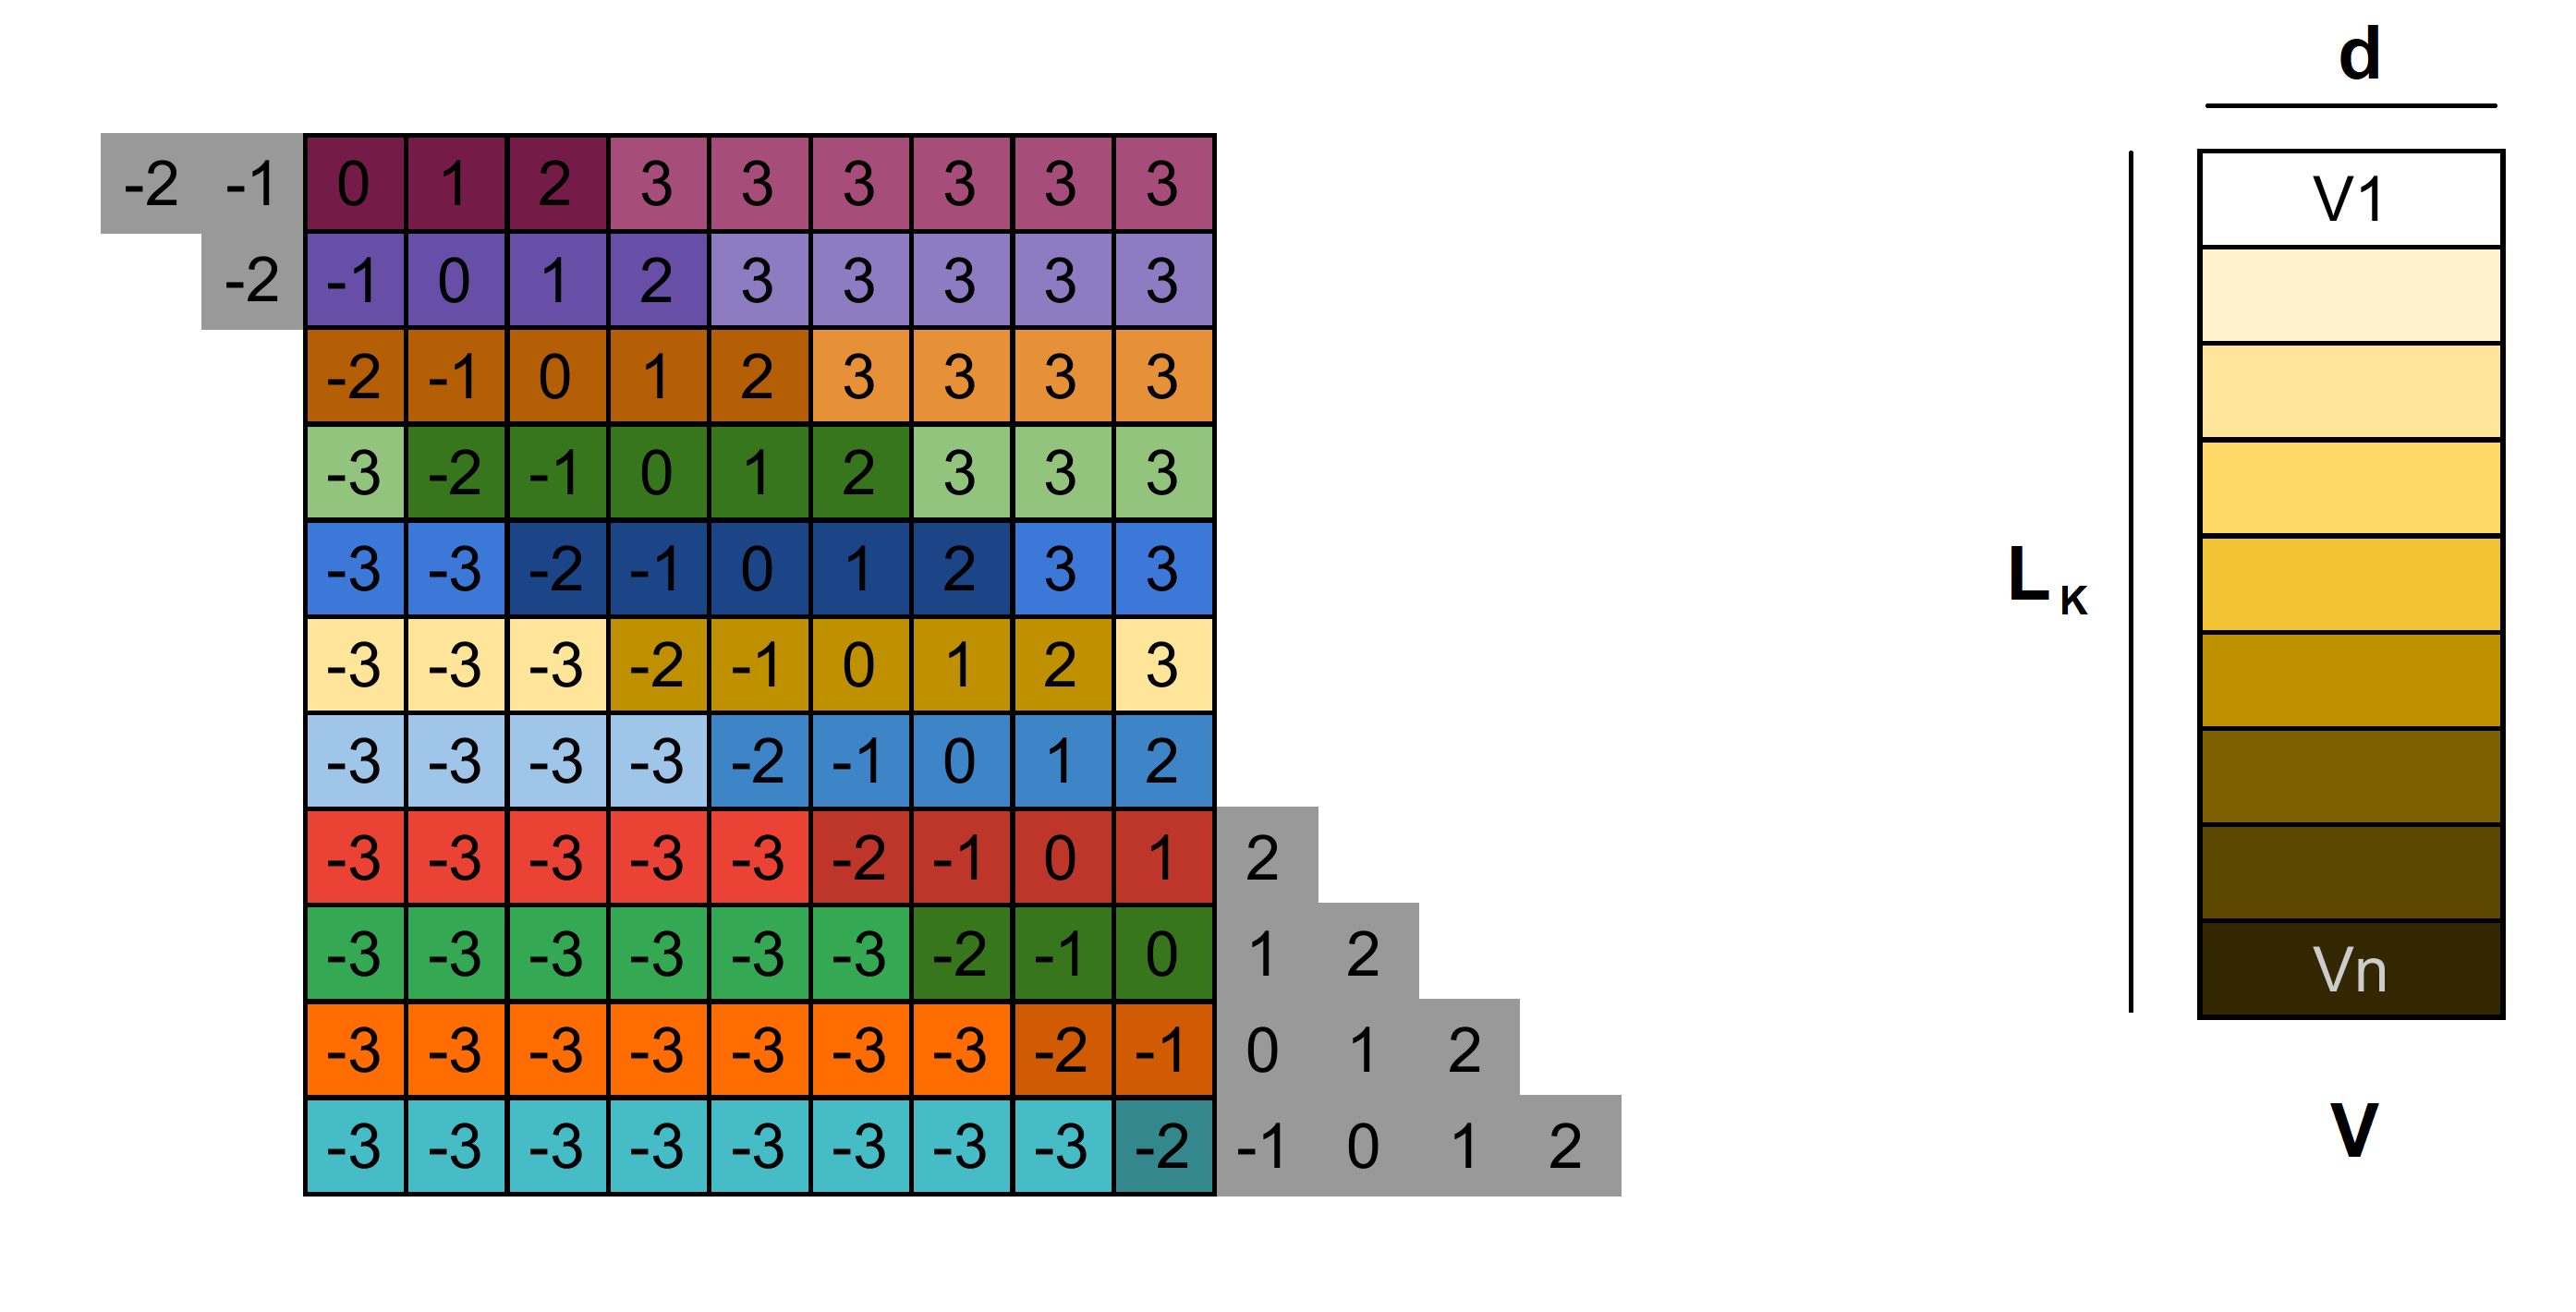
\includegraphics[width=0.9\linewidth]{images/S_rel_V.png}
\caption{$A_{rel}$ calculation}
\label{fig:A_rel_naive}
\end{figure}

One can observe in figure \ref{fig:A_rel_naive} that some weights are repeated several times in the
$S_{rel}$ matrix. Calculating the whole matrix can be avoided by
instead calculating all possible weights only once, with complexity
$O \left(L_Q\times d\times(2k+1)\right)$). As illustrated in figure \ref{fig:A_rel_linear}, the matrix multiplication can then be replaced by a sum of three terms. The embedding dimension of size $d$ is not represented here. Instead the horizontal axis in the figure represents all terms that must be summed. The grey squares represent some zero-padding. The first term is a cumulated sum of the value vectors that is weighted  by the before-horizon set of weights (complexity $O(max(L_Q, L_K))$). The second term is a weighed sum of a moving window of the value vectors. Where the weights are the central diagonal of the $S_{rel}$ matrix. (complexity $O(L_Q \times (2k-1) \times d)$). The last term is similar to the first term, but for the after-horizon set of weights (complexity $O(max(L_Q, L_K))$). The implementation is given in algorithm \ref{alg:A_rel}. The algorithm is given for bidirectional attention only, but it can easily be adapted for masked attention.

\begin{figure}
\centering
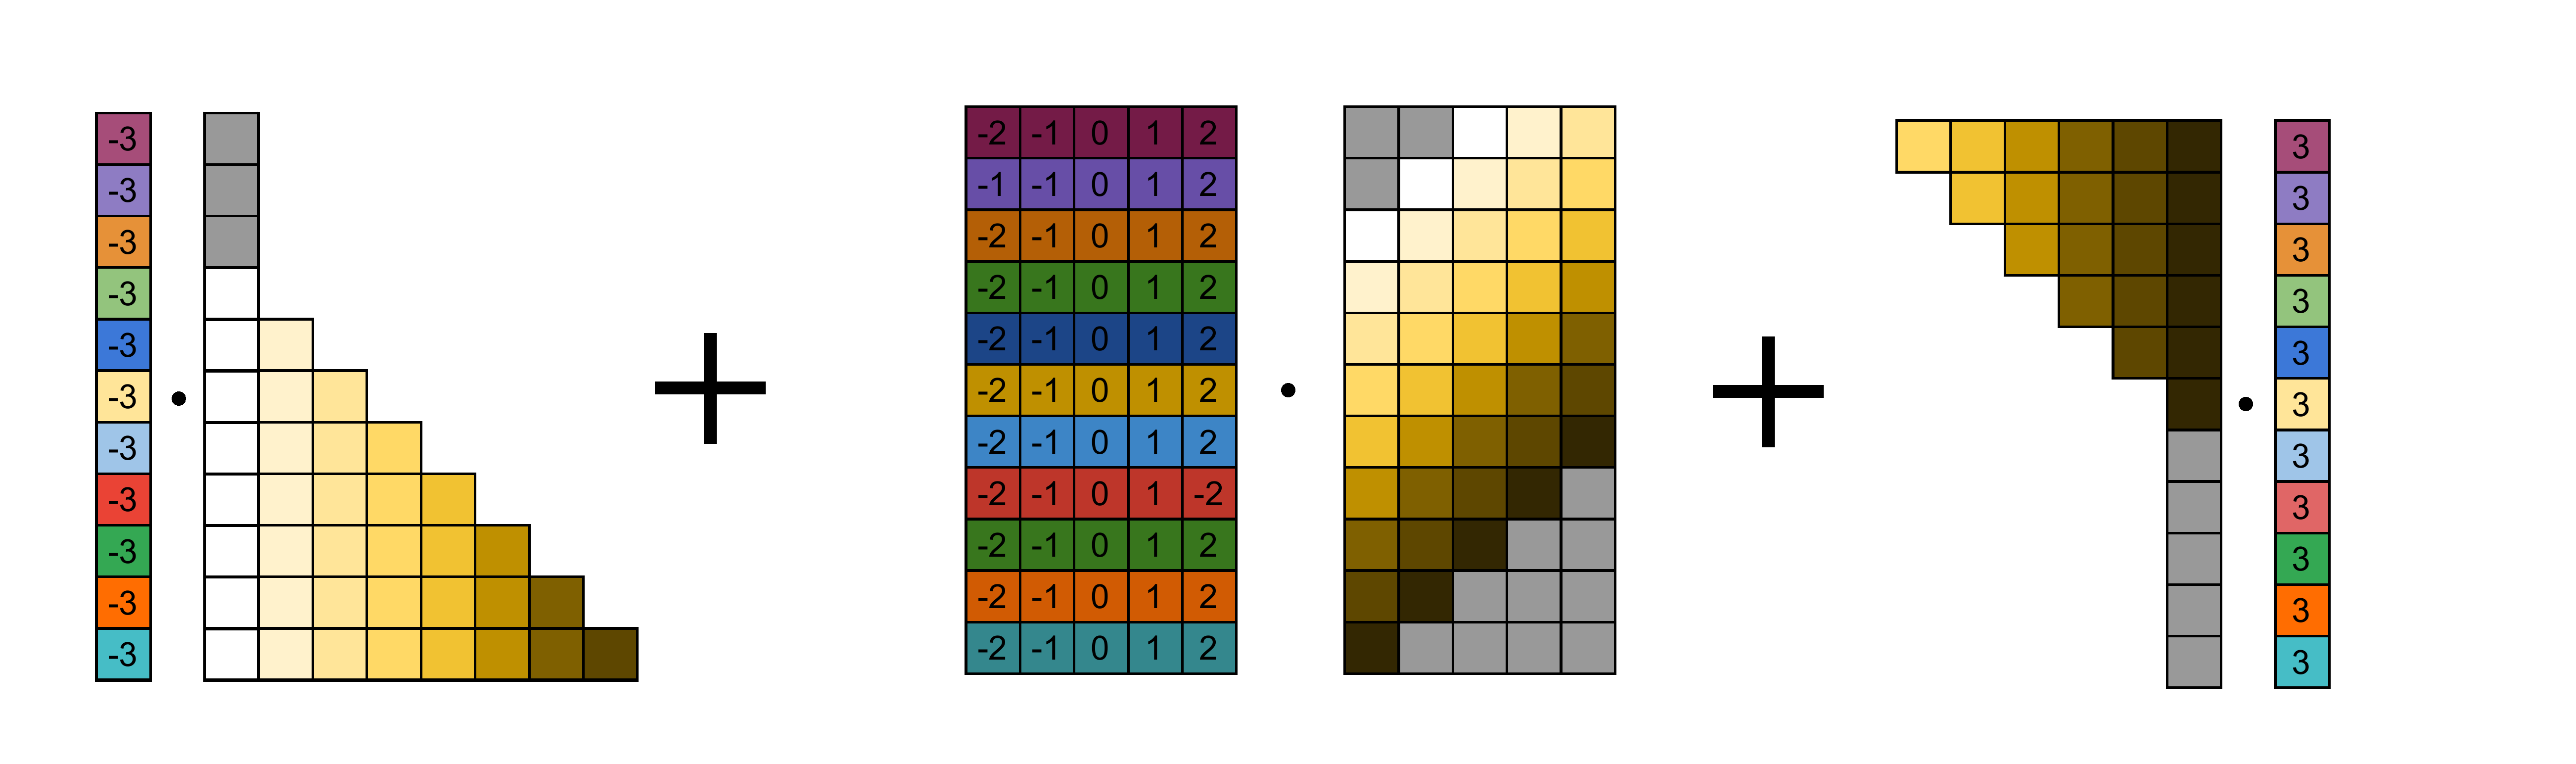
\includegraphics[width=0.9\linewidth]{images/S_rel_V_detailed.png}
\caption{$A_{rel}$ simplified calculation}
\label{fig:A_rel_linear}
\end{figure}

\begin{algorithm}[H]
	\caption{calculation of $A_{rel}$ with linear complexity}
	\label{alg:A_rel}
	\KwData{$\phi(Q)$, $RP$, $V$ tensors of shape $(L_Q, d)$, $(2k+1, d)$, and $(L_K, d)$}
	\KwResult{$A_{rel}$ tensor of shape $(L_Q, d)$}
	$W := \phi(Q) \times RP^T$\\
	$W_{before} := W_{[:, 0]}$\\
	$n_{before} := min(max(0, L_Q-k), L_K)$\\
	$\text{Padding}_{before} := zeros(min(k, L_Q), d)$\\
	$\text{Padded}_{before} := concatenate(\text{Padding}_{before}, cumsum(V))$\\
	$V_{before} := aligned(\text{Padded}_{before}, n_{before})$\\
	$W_{horizon} := W_{[:, 1:2k-1]}$\\
	$V^{horizon} := zeros(L_Q, 2k-1, d)$\\
	\For{$i=0$ \KwTo $L_Q-1$}
	{
		\For{$j=0$ \KwTo $2k-2$}
		{
			\For{$l=0$ \KwTo $d-1$}
			{
					$V^{horizon}_{ijl} =
					\begin{cases}
						V_{[i-k+1+j, l]}\text{ if }0 \leq (i-k+1+j) < L_K\\
						0\text{ otherwise} 
					\end{cases}$
			}
		}
	}
	$W_{after} := W_{[:, 2k]}$\\
	$n_{after} := min(L_Q+k, L_K)$\\
	$\text{Summed} := sum(V[k-1:n_{after}, :], \text{dim=0})$\\
	$\text{rCumSum} := \text{Summed} - cumsum(V[k-1:n_{after}-1, :])$\\
	$\text{Padding}_{after} := zeros(max(0, Lq-max(0, Lk-R)), D)$\\
	$V_{after} := concatenate(\text{rCumSum}, \text{Padding}_{after})$\\
	$A_{rel} := W_{before} \cdot V_{before} + sum(W_{horizon} \cdot V^{horizon}, \text{dim=1}) + W_{after} \cdot V_{after}$
\end{algorithm}

\endinput
